% ============================================================================
% Kiến trúc tổng quát Mobile-U-ViT — TikZ diagram
% Biên dịch: pdflatex (cần package tikz)
% ============================================================================
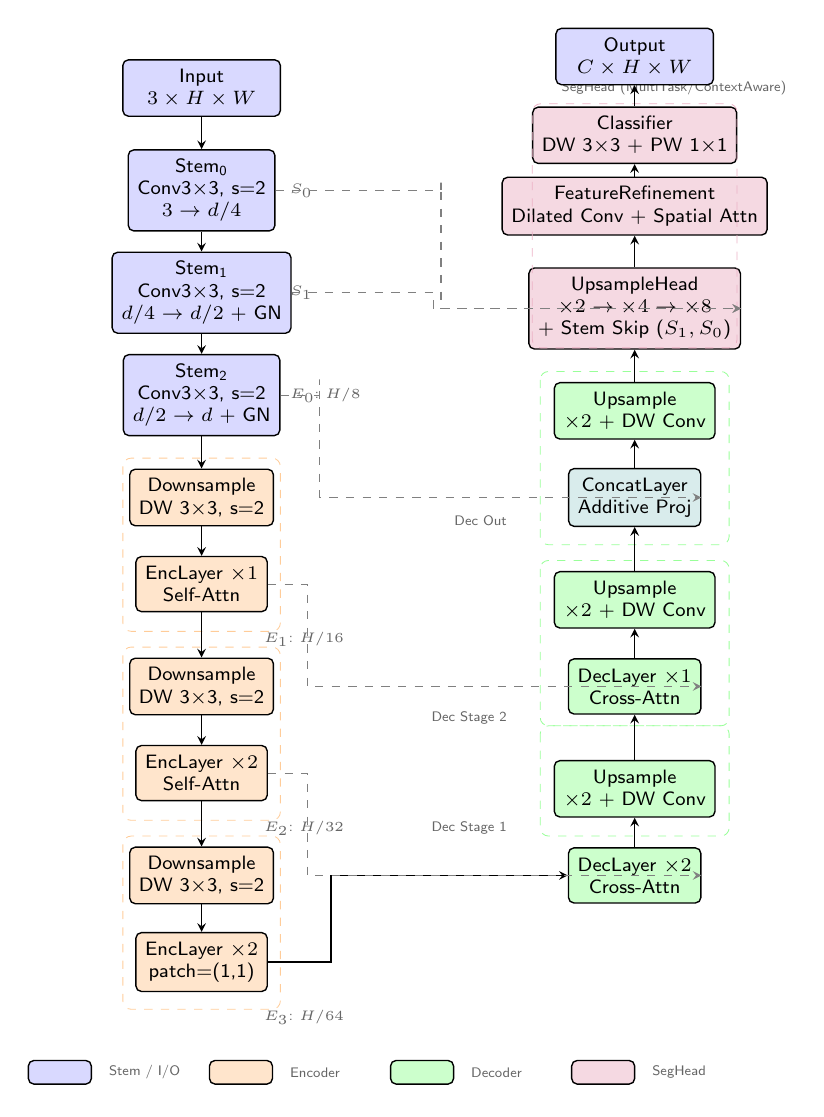
\begin{tikzpicture}[
    % ── Style definitions ──
    block/.style={
        rectangle, draw=black, line width=0.5pt,
        minimum width=1.6cm, minimum height=0.55cm,
        align=center, font=\scriptsize\sffamily,
        rounded corners=2pt,
    },
    stem/.style={block, fill=blue!15},
    enc/.style={block, fill=orange!20},
    dec/.style={block, fill=green!20},
    head/.style={block, fill=purple!15},
    attn/.style={block, fill=red!10},
    concat/.style={block, fill=teal!15},
    arrow/.style={->, >=stealth, line width=0.4pt},
    skip/.style={->, >=stealth, line width=0.4pt, dashed, gray},
    box/.style={rectangle, draw=black!40, line width=0.3pt, dashed, rounded corners=3pt},
    lbl/.style={font=\tiny\sffamily, text=black!60},
]

% ═══════════════════════════════════════════════════════════════
% INPUT
% ═══════════════════════════════════════════════════════════════
\node[stem, minimum width=2.0cm] (input) at (0, 10.5) {Input\\$3 \times H \times W$};

% ═══════════════════════════════════════════════════════════════
% STEM (3 tầng)
% ═══════════════════════════════════════════════════════════════
\node[stem] (stem0) at (0, 9.2) {Stem\textsubscript{0}\\Conv3$\times$3, s=2\\$3\to d/4$};
\node[stem] (stem1) at (0, 7.9) {Stem\textsubscript{1}\\Conv3$\times$3, s=2\\$d/4\to d/2$ + GN};
\node[stem] (stem2) at (0, 6.6) {Stem\textsubscript{2}\\Conv3$\times$3, s=2\\$d/2\to d$ + GN};

% Stem outputs annotation
\node[lbl, anchor=west] at (1.0, 9.2) {$S_0$};
\node[lbl, anchor=west] at (1.0, 7.9) {$S_1$};

% ═══════════════════════════════════════════════════════════════
% ENCODER (3 stage)
% ═══════════════════════════════════════════════════════════════
% Stage 1
\node[enc] (enc1_ds) at (0, 5.3) {Downsample\\DW 3$\times$3, s=2};
\node[enc, minimum height=0.7cm] (enc1_l) at (0, 4.2) {EncLayer $\times 1$\\Self-Attn};

% Stage 2
\node[enc] (enc2_ds) at (0, 2.9) {Downsample\\DW 3$\times$3, s=2};
\node[enc, minimum height=0.7cm] (enc2_l) at (0, 1.8) {EncLayer $\times 2$\\Self-Attn};

% Stage 3
\node[enc] (enc3_ds) at (0, 0.5) {Downsample\\DW 3$\times$3, s=2};
\node[enc, minimum height=0.7cm] (enc3_l) at (0, -0.6) {EncLayer $\times 2$\\patch=(1,1)};

% Encoder stage boxes
\draw[box, orange!40] (-1.0, 5.8) rectangle (1.0, 3.6);
\node[lbl] at (1.3, 3.5) {$E_1$: $H/16$};

\draw[box, orange!40] (-1.0, 3.4) rectangle (1.0, 1.2);
\node[lbl] at (1.3, 1.1) {$E_2$: $H/32$};

\draw[box, orange!40] (-1.0, 1.0) rectangle (1.0, -1.2);
\node[lbl] at (1.3, -1.3) {$E_3$: $H/64$};

% Encoder annotations
\node[lbl, anchor=west] at (1.0, 6.6) {$E_0$: $H/8$};

% ═══════════════════════════════════════════════════════════════
% DECODER (3 stage) — bên phải, mirror encoder
% ═══════════════════════════════════════════════════════════════

% Stage 1 (decoder) — xử lý từ dưới lên
\node[dec, minimum height=0.7cm] (dec1_l) at (5.5, 0.5) {DecLayer $\times 2$\\Cross-Attn};
\node[dec] (dec1_us) at (5.5, 1.6) {Upsample\\$\times 2$ + DW Conv};

% Stage 2
\node[dec, minimum height=0.7cm] (dec2_l) at (5.5, 2.9) {DecLayer $\times 1$\\Cross-Attn};
\node[dec] (dec2_us) at (5.5, 4.0) {Upsample\\$\times 2$ + DW Conv};

% Out block
\node[concat, minimum height=0.7cm] (dec3_l) at (5.5, 5.3) {ConcatLayer\\Additive Proj};
\node[dec] (dec3_us) at (5.5, 6.4) {Upsample\\$\times 2$ + DW Conv};

% Decoder stage boxes
\draw[box, green!40] (4.3, 2.4) rectangle (6.7, 1.0);
\node[lbl, anchor=east] at (4.0, 1.1) {Dec Stage 1};

\draw[box, green!40] (4.3, 4.5) rectangle (6.7, 2.4);
\node[lbl, anchor=east] at (4.0, 2.5) {Dec Stage 2};

\draw[box, green!40] (4.3, 6.9) rectangle (6.7, 4.7);
\node[lbl, anchor=east] at (4.0, 5.0) {Dec Out};

% ═══════════════════════════════════════════════════════════════
% SEG HEAD
% ═══════════════════════════════════════════════════════════════
\node[head] (seg_us) at (5.5, 7.7) {UpsampleHead\\$\times 2 \to \times 4 \to \times 8$\\+ Stem Skip ($S_1,S_0$)};
\node[head, minimum height=0.7cm] (seg_ref) at (5.5, 9.0) {FeatureRefinement\\Dilated Conv + Spatial Attn};
\node[head, minimum height=0.6cm] (seg_cls) at (5.5, 9.9) {Classifier\\DW 3$\times$3 + PW 1$\times$1};

\draw[box, purple!30] (4.2, 7.2) rectangle (6.8, 10.3);
\node[lbl] at (6.0, 10.5) {SegHead (MultiTask/ContextAware)};

% Output
\node[stem, minimum width=2.0cm] (output) at (5.5, 10.9) {Output\\$C \times H \times W$};

% ═══════════════════════════════════════════════════════════════
% ARROWS — Main forward path
% ═══════════════════════════════════════════════════════════════

% Input → Stem
\draw[arrow] (input) -- (stem0);
\draw[arrow] (stem0) -- (stem1);
\draw[arrow] (stem1) -- (stem2);

% Stem → Encoder
\draw[arrow] (stem2) -- (enc1_ds);
\draw[arrow] (enc1_ds) -- (enc1_l);
\draw[arrow] (enc1_l) -- (enc2_ds);
\draw[arrow] (enc2_ds) -- (enc2_l);
\draw[arrow] (enc2_l) -- (enc3_ds);
\draw[arrow] (enc3_ds) -- (enc3_l);

% Latent → Decoder (bottom connection)
\draw[arrow] (enc3_l.east) -- ++(0.8, 0) |- (dec1_l.west);

% Decoder upward
\draw[arrow] (dec1_l) -- (dec1_us);
\draw[arrow] (dec1_us) -- (dec2_l);
\draw[arrow] (dec2_l) -- (dec2_us);
\draw[arrow] (dec2_us) -- (dec3_l);
\draw[arrow] (dec3_l) -- (dec3_us);

% Decoder → SegHead
\draw[arrow] (dec3_us) -- (seg_us);
\draw[arrow] (seg_us) -- (seg_ref);
\draw[arrow] (seg_ref) -- (seg_cls);
\draw[arrow] (seg_cls) -- (output);

% ═══════════════════════════════════════════════════════════════
% SKIP CONNECTIONS (Encoder → Decoder)
% ═══════════════════════════════════════════════════════════════

% E_2 → Dec Stage 1 (cross-attention memory)
\draw[skip] (enc2_l.east) -- ++(0.5, 0) -- ++(0, -0.5) |- (dec1_l.east);

% E_1 → Dec Stage 2 (cross-attention memory)
\draw[skip] (enc1_l.east) -- ++(0.5, 0) -- ++(0, -0.5) |- (dec2_l.east);

% E_0 → Dec Out (ConcatLayer memory)
\draw[skip] (stem2.east) -- ++(0.5, 0) -- ++(0, +0.2) |- (dec3_l.east);

% ═══════════════════════════════════════════════════════════════
% STEM SKIPS (Stem → UpsampleHead)
% ═══════════════════════════════════════════════════════════════
\draw[skip] (stem1.east) -- ++(1.8, 0) -- ++(0, -0.1) |- (seg_us.east);
\draw[skip] (stem0.east) -- ++(2.1, 0) -- ++(0, +0.1) |- (seg_us.east);

% ═══════════════════════════════════════════════════════════════
% LEGEND
% ═══════════════════════════════════════════════════════════════
\node[stem, minimum width=0.8cm, minimum height=0.3cm, font=\tiny] at (-1.8, -2.0) {};
\node[lbl, anchor=west] at (-1.3, -2.0) {Stem / I/O};
\node[enc, minimum width=0.8cm, minimum height=0.3cm, font=\tiny] at (0.5, -2.0) {};
\node[lbl, anchor=west] at (1.0, -2.0) {Encoder};
\node[dec, minimum width=0.8cm, minimum height=0.3cm, font=\tiny] at (2.8, -2.0) {};
\node[lbl, anchor=west] at (3.3, -2.0) {Decoder};
\node[head, minimum width=0.8cm, minimum height=0.3cm, font=\tiny] at (5.1, -2.0) {};
\node[lbl, anchor=west] at (5.6, -2.0) {SegHead};

\end{tikzpicture}
